\subsection{Rate Encoding}

In rate encoding, the objective is to represent each feature pixel of an image as a sequence of discrete values, \(x_{i,j} \in \{0, 1\}\), while converting the image into a time-varying sequence of spikes that retain a relation to the original image. This process involves using a normalization function \(f: \mathbb{R} \rightarrow [0, 1]\) to map the input image \(x\) to a firing rate value \(p\) in the range \([0, 1]\) that is used to generate a stochastic spike sequence \(S_{i,j}\) using a chosen distribution \(D\).

One common implementation is to use the binomial distribution \(D = \text{Bin}(n, p)\), where \(n\) is the number of time samples, and \(p\) is an adjustable parameter according to the input value. The relationship between \(p\) and \(f(x_{i,j})\) is given by:

\begin{equation}
    p = f(x_{i,j}) \cdot F_0 \cdot \Delta t 
\end{equation}

where \(F_0\) is the maximum firing rate (20 Hz), and \(\Delta t\) is the time interval between consecutive samples. This equation allows us to set the expectancy \(E[D(x_{i,j})]\) for each \(x_{i,j}\) to \(f(x_{i,j}) \cdot F_0 \cdot T\), where \(T\) is the experiment time.

By using this derived equation, we can implement the rate encoding approach in a way that controls the spike generation based on the input image and ensures that high-intensity pixels (corresponding to higher values of \(f(x_{i,j})\)) will appear in more patterns.

Overall, the rate encoding approach, combined with the derived probability constraints and stochastic spike generation, enables us to effectively convert an image into a time-varying sequence of spikes while preserving its features. This method allows us to model the behavior of real neurons and capture the temporal dynamics of the input information, making it suitable for various applications in neural information processing and spiking neural network simulations.

\begin{figure}[H]
    \centering
    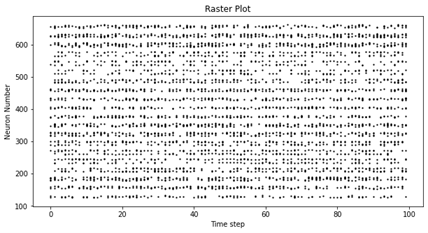
\includegraphics[width=0.5\textwidth]{methods/spike-encoding/graphs/rate-encoding-raster.png}
    \caption{Raster plot of a random Mnist image encoded via Rate Encoding with maximum rate of 20 Hz over trial time of 1 sec}
    \label{fig:rate-encoding-raster}
\end{figure}
